\documentclass[aspectratio=169,t,xcolor=table]{beamer}
\usepackage[utf8]{inputenc}
\usepackage[brazil]{babel}
\usepackage{booktabs}
\usepackage{tabularx}
\usepackage{listings}
\usepackage{graphicx}

\usetheme{Ufg}
\usetikzlibrary{positioning}

\graphicspath{{../assets/}{assets/}{figs/}}

\setbeamertemplate{caption}[numbered]

\AtBeginSection[]{%
    \setLayout{mainpoint}%
    \setBGColor{\currentsectioncolor}%
    \begin{frame}[noframenumbering]{}%
        \frametitle{\insertsectionhead}%
    \end{frame}%
    \setLayout{vertical}%
}

\setPrimaryColor{UFGBlue}
\setLogos{lib/logos/INF-compact-white.png}{lib/logos/INF-compact-white.png}

\title[Sistema de Agendamento --- APS 1]{Sistema de Agendamento de Consultas Médicas}
\subtitle{Modelagem de Software --- APS 1 (Especificação UML)}
\author[Grupo 5]{%
  Carlos Eduardo Freire \and Gabriel Henrique Lourenço \and Kayque Vicente Silva\\
  Luiz Pedro Pereira Mendes \and Yury Nogueira de Oliveira%
}
\institute[UFG/INF]{%
  Instituto de Informática (INF) --- Universidade Federal de Goiás (UFG)\\
  Bacharelado em Engenharia de Software --- Docente: Me. Diogo Oliveira Santos%
}
\date{2026/2}

\begin{document}

% Slide 1: Capa
\frame[noframenumbering]{\titlepage}

% Slide 2: Identificação do Grupo e Contexto
\setLayout{horizontal}
\begin{frame}{Identificação Acadêmica e Equipe}
    \begin{columns}
        \column{0.52\textwidth}
        \textbf{Contexto da Atividade:}
        \begin{itemize}
            \item \textbf{Disciplina:} Modelagem de Software (APS 1)
            \item \textbf{Instituição:} Instituto de Informática (INF / UFG)
            \item \textbf{Curso:} Bacharelado em Engenharia de Software
            \item \textbf{Docente:} Me. Diogo Oliveira Santos
            \item \textbf{Semestre Letivo:} 2026/2
        \end{itemize}

        \column{0.48\textwidth}
        \textbf{Integrantes do Grupo:}
        \begin{itemize}
            \item Carlos Eduardo Freire da Silva
            \item Gabriel Henrique Lourenço Dias
            \item Kayque Vicente Silva
            \item Luiz Pedro Pereira Mendes Saraiva
            \item Yury Nogueira de Oliveira Silva
        \end{itemize}
    \end{columns}
\end{frame}

% Slide 3: Agenda
\setLayout{vertical}
\begin{frame}{Agenda da Apresentação}
    \tableofcontents
\end{frame}

% ==========================================================
\section[UFGBlue]{Visão Geral e Requisitos}

% Slide 4: Problema de Negócio e Solução
\setLayout{horizontal}
\begin{frame}{Problema de Negócio e Solução Proposta}
    \begin{columns}
        \column{0.5\textwidth}
        \textbf{Desafios Operacionais:}
        \begin{itemize}
            \item Conflitos e sobreposição de horários na recepção
            \item Alto índice de faltas por ausência de lembretes
            \item Morosidade no cancelamento e na remarcação
            \item Falta de rastreabilidade e auditoria (LGPD)
        \end{itemize}

        \column{0.5\textwidth}
        \textbf{Solução Modelada:}
        \begin{itemize}
            \item Autoatendimento integrado para pacientes
            \item Reserva com controle estrito de concorrência
            \item Notificações paralelas via E-mail e WhatsApp
            \item Log imutável para eventos críticos de negócio
        \end{itemize}
    \end{columns}
\end{frame}

% Slide 5: Atores do Sistema
\setLayout{horizontal}
\begin{frame}{Atores e Perfis de Acesso}
    \begin{columns}
        \column{0.5\textwidth}
        \begin{block}{Paciente (Autoatendimento)}
            Pesquisa especialidades e médicos, agenda horários livres, cancela e solicita remarcações.
        \end{block}
        \vspace{0.6em}
        \begin{block}{Médico (Corpo Clínico)}
            Configura disponibilidade semanal, visualiza agenda do dia, inicia atendimentos e encerra consultas.
        \end{block}

        \column{0.5\textwidth}
        \begin{block}{Secretário (Recepção)}
            Atendimento presencial/telefônico, confirmação ativa de agendamentos e bloqueios operacionais.
        \end{block}
        \vspace{0.6em}
        \begin{block}{Administrador (Gestão)}
            Gerenciamento global de usuários, médicos, clínicas, especialidades e relatórios de auditoria.
        \end{block}
    \end{columns}
\end{frame}

% Slide 6: Ciclo de Vida da Consulta
\setLayout{vertical}
\begin{frame}{Ciclo de Vida da Consulta}
    \centering
    \resizebox{\textwidth}{!}{%
    \begin{tabular}{llll}
        \toprule
        \textbf{Estado Atual} & \textbf{Evento / Ação} & \textbf{Novo Estado} & \textbf{Ator Responsável} \\
        \midrule
        --- & Solicitar agendamento & \texttt{AGENDADA} & Paciente / Secretário \\
        \texttt{AGENDADA} & Confirmar presença & \texttt{CONFIRMADA} & Secretário / Médico \\
        \texttt{AGENDADA / CONFIRMADA} & Iniciar atendimento & \texttt{EM\_ANDAMENTO} & Médico titular \\
        \texttt{EM\_ANDAMENTO} & Concluir atendimento & \texttt{REALIZADA} & Médico titular \\
        \texttt{AGENDADA / CONFIRMADA} & Cancelar ($\ge$ 2 h com motivo) & \texttt{CANCELADA} & Paciente / Secretário \\
        \texttt{AGENDADA / CONFIRMADA} & Remarcar ($\ge$ 2 h com motivo) & \texttt{REMARCADA} (nova \texttt{AGENDADA}) & Paciente / Secretário \\
        \texttt{AGENDADA / CONFIRMADA} & Ausência / Não comparecimento & \texttt{NAO\_REALIZADA} & Médico / Sistema automático \\
        \bottomrule
    \end{tabular}%
    }
    \vspace{0.8em}
    \begin{itemize}
        \item \textbf{Estados Finais:} \texttt{REALIZADA}, \texttt{CANCELADA}, \texttt{REMARCADA} e \texttt{NAO\_REALIZADA}.
        \item \textbf{Regra de Negócio (RN-20):} Cancelamento e remarcação exigem no mínimo 2 horas de antecedência.
    \end{itemize}
\end{frame}

% Slide 7: Notificações e Regras Críticas
\setLayout{horizontal}
\begin{frame}{Notificações Multicanal e Concorrência}
    \begin{columns}
        \column{0.5\textwidth}
        \textbf{Comunicação em 2 Canais:}
        \begin{itemize}
            \item Disparos assíncronos por E-mail e WhatsApp
            \item Eventos: Agendamento, Confirmação, Cancelamento, Remarcação e Lembrete (24 h)
            \item Fila com até 3 tentativas e espaçamento progressivo
            \item Falha no envio não compromete o agendamento
        \end{itemize}

        \column{0.5\textwidth}
        \textbf{Restrições e Auditoria:}
        \begin{itemize}
            \item Janela mínima de 30 minutos e máxima de 90 dias
            \item Slots padrões de 30 minutos sem sobreposição
            \item Bloqueio de horários com justificativa obrigatória
            \item Log imutável de auditoria com rastreio de IP e autor
        \end{itemize}
    \end{columns}
\end{frame}

% ==========================================================
\section[Ocean]{Diagrama de Atividades (DA-01)}

% Slide 8: DA-01 Imagem
\setLayout{vertical}
\begin{frame}{DA-01 --- Agendamento de Consulta}
    \centering
    \vspace{0.1cm}
    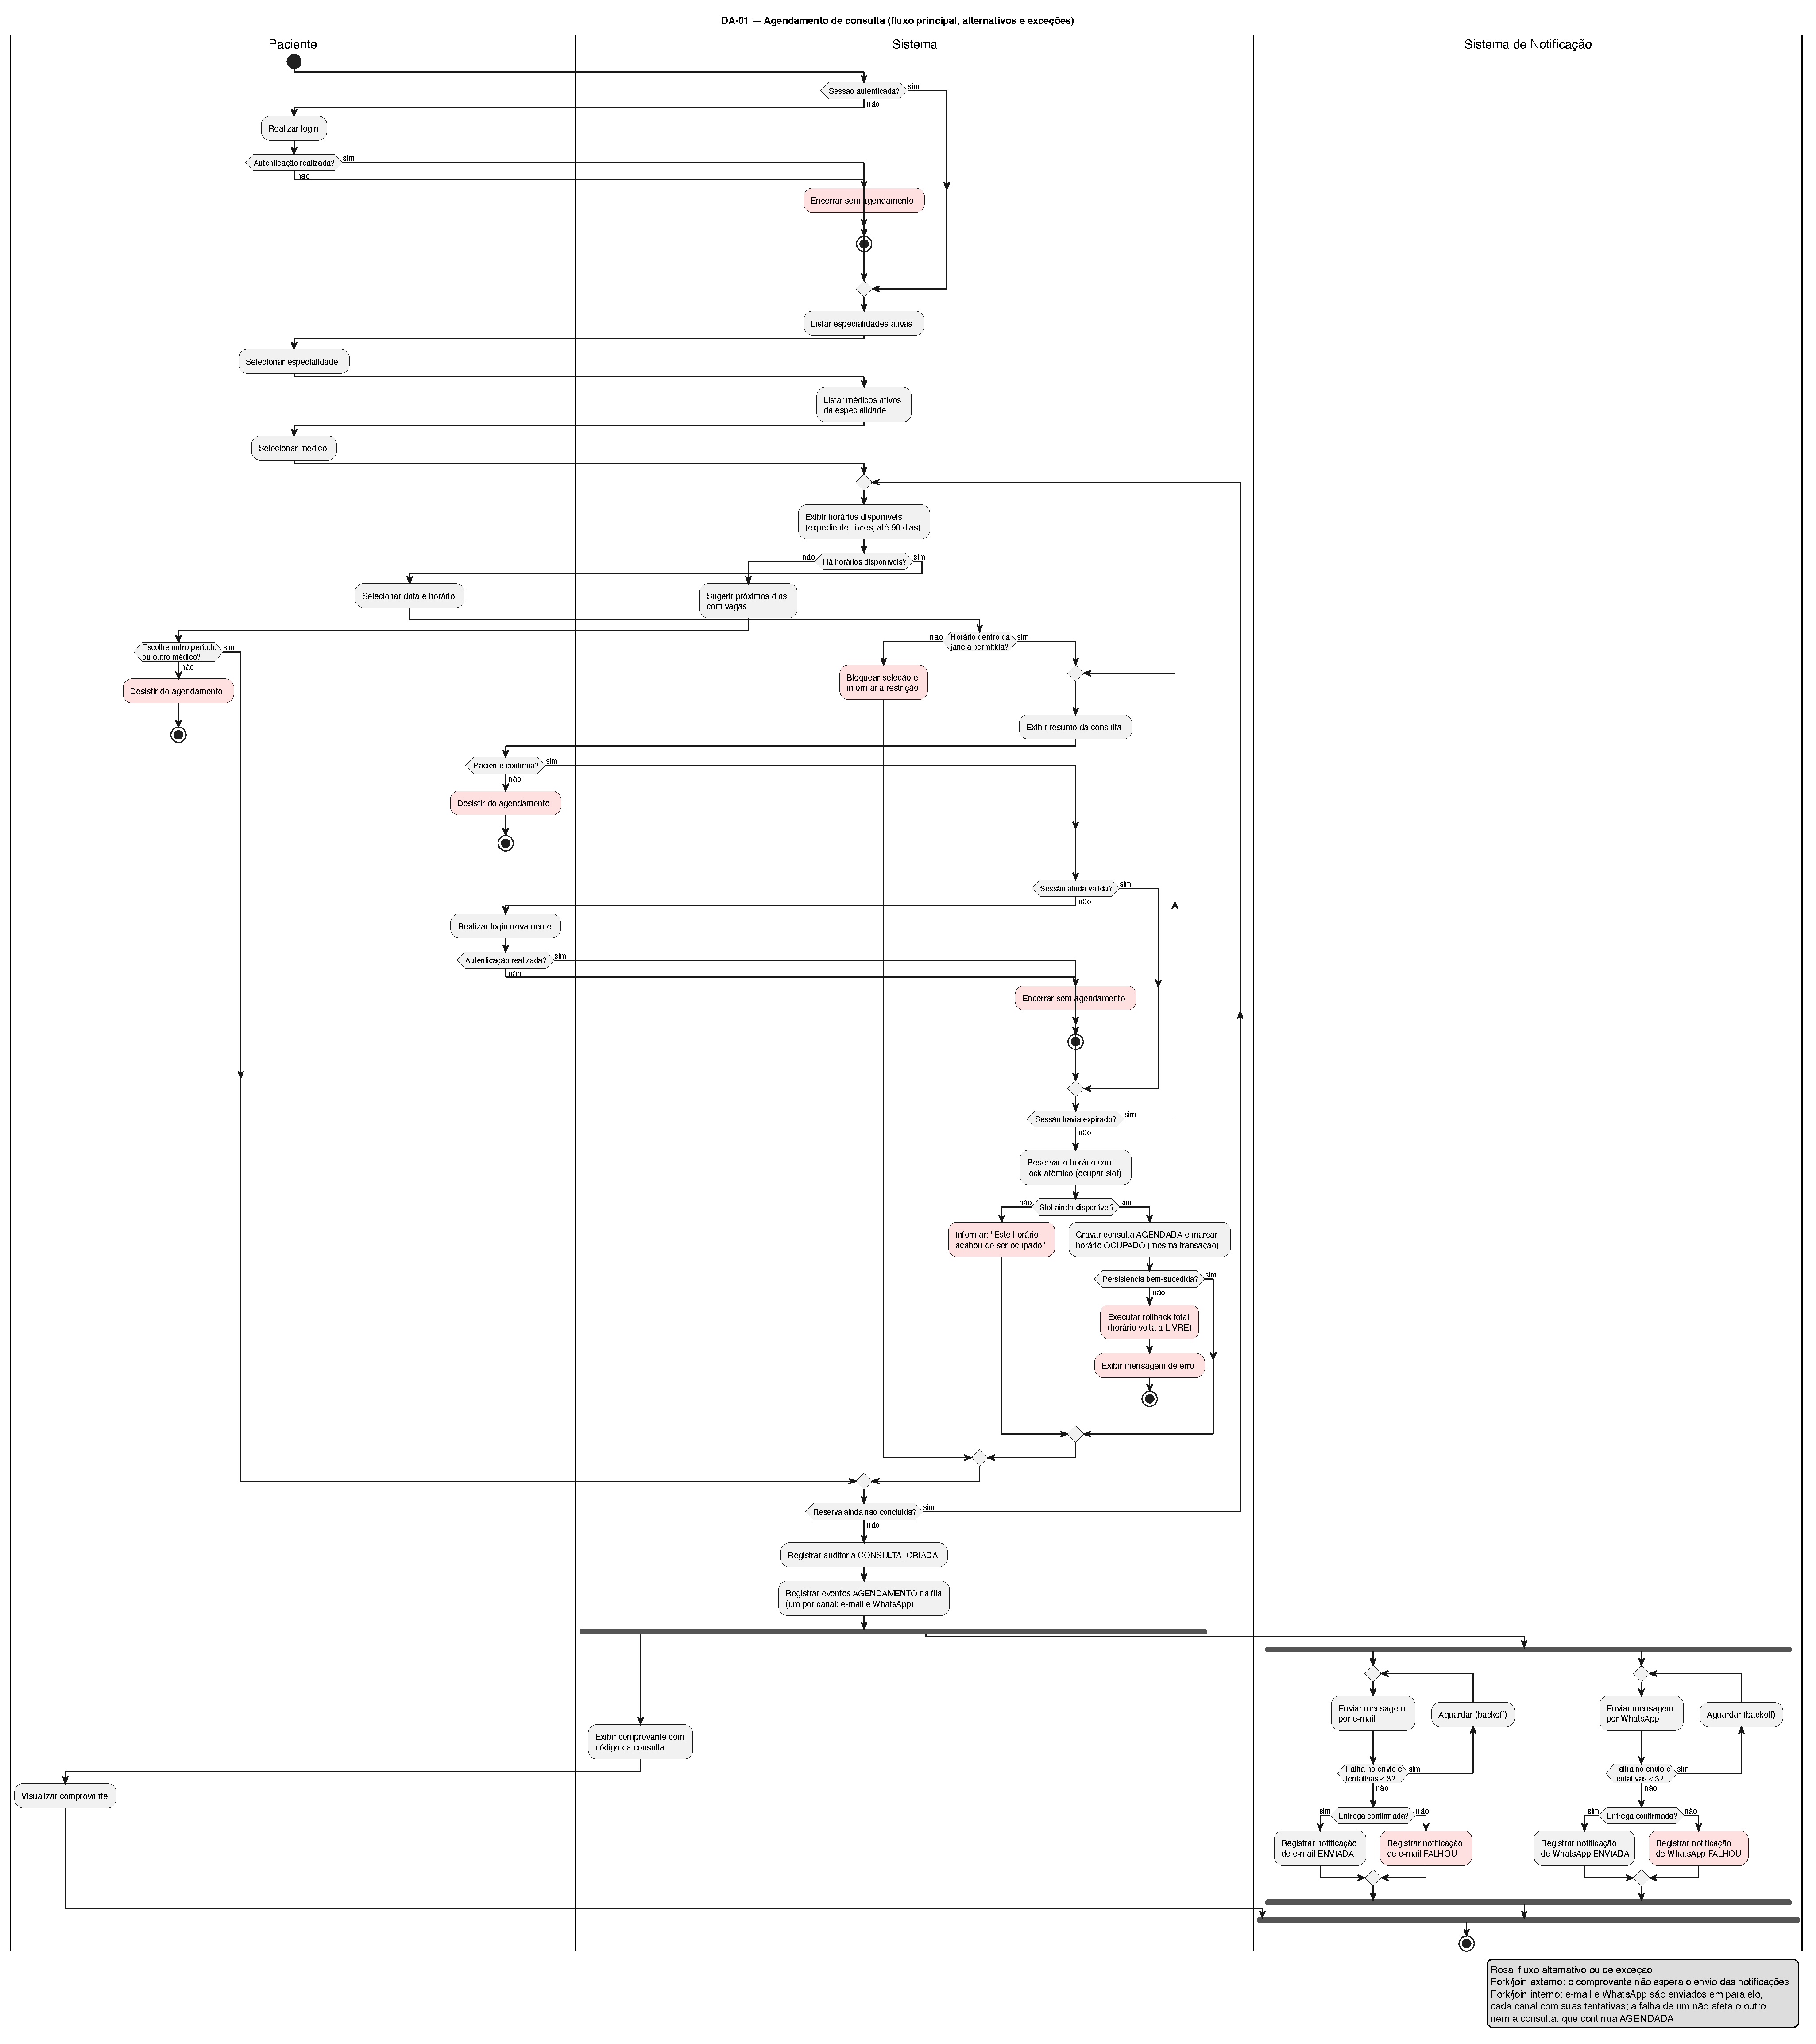
\includegraphics[width=\textwidth,height=5.8cm,keepaspectratio]{DA01_Agendamento.pdf}
\end{frame}

% Slide 9: DA-01 Mecânica Operacional
\setLayout{horizontal}
\begin{frame}{DA-01 --- Mecânica Operacional e Concorrência}
    \begin{columns}
        \column{0.5\textwidth}
        \textbf{Organização em Raias:}
        \begin{itemize}
            \item \textbf{Paciente:} autenticação, seleção e confirmação
            \item \textbf{Sistema:} validação, reserva atômica e auditoria
            \item \textbf{Notificação:} processamento assíncrono paralelo
        \end{itemize}
        \vspace{0.5em}
        \textbf{Desacoplamento por Fork/Join:}
        \begin{itemize}
            \item Comprovante emitido de forma imediata
            \item Paciente não aguarda resposta das operadoras
        \end{itemize}

        \column{0.5\textwidth}
        \textbf{Prevenção de Colisões:}
        \begin{itemize}
            \item Bloqueio instantâneo do slot na confirmação
            \item Repetição (\texttt{repeat}) em horários tomados
            \item Sugestão de novas datas em ausência de vagas
        \end{itemize}
        \vspace{0.5em}
        \textbf{Mecanismo de Rollback:}
        \begin{itemize}
            \item Em falha de gravação, o horário volta a \texttt{LIVRE}
        \end{itemize}
    \end{columns}
\end{frame}

% Slide 10: DA-01 Tabela de Fluxos Alternativos
\setLayout{vertical}
\begin{frame}{DA-01 --- Mapeamento de Exceções e Desvios}
    \centering
    \resizebox{\textwidth}{!}{%
    \begin{tabular}{lp{10.5cm}}
        \toprule
        \textbf{Identificador} & \textbf{Tratamento no Fluxo do Diagrama} \\
        \midrule
        \textbf{A1 --- Sem Horários} & Sugestão automática de datas alternativas pelo sistema; permite reescolha ou saída. \\
        \textbf{A2 --- Conflito no Slot} & Horário ocupado concorrentemente; emite aviso amigável e retorna à seleção. \\
        \textbf{A3 --- Falha de Notificação} & Até 3 tentativas automáticas por canal; se esgotar, marca \texttt{FALHOU} sem desfazer a consulta. \\
        \textbf{E1 --- Sessão Expirada} & Solicita reautenticação imediata e restaura o resumo previamente preenchido. \\
        \textbf{E2 --- Erro de Persistência} & Falha ao gravar no banco; cancela operação, libera o slot (\texttt{LIVRE}) e alerta o usuário. \\
        \textbf{E3 --- Fora da Janela} & Seleção anterior a 30 min ou posterior a 90 dias; bloqueia seleção com mensagem clara. \\
        \bottomrule
    \end{tabular}%
    }
\end{frame}

% ==========================================================
\section[DarkPurple]{Diagrama de Sequência (DS-01)}

% Slide 11: DS-01 Imagem
\setLayout{vertical}
\begin{frame}{DS-01 --- Agendamento de Consulta (Fluxo Completo)}
    \centering
    \vspace{0.1cm}
    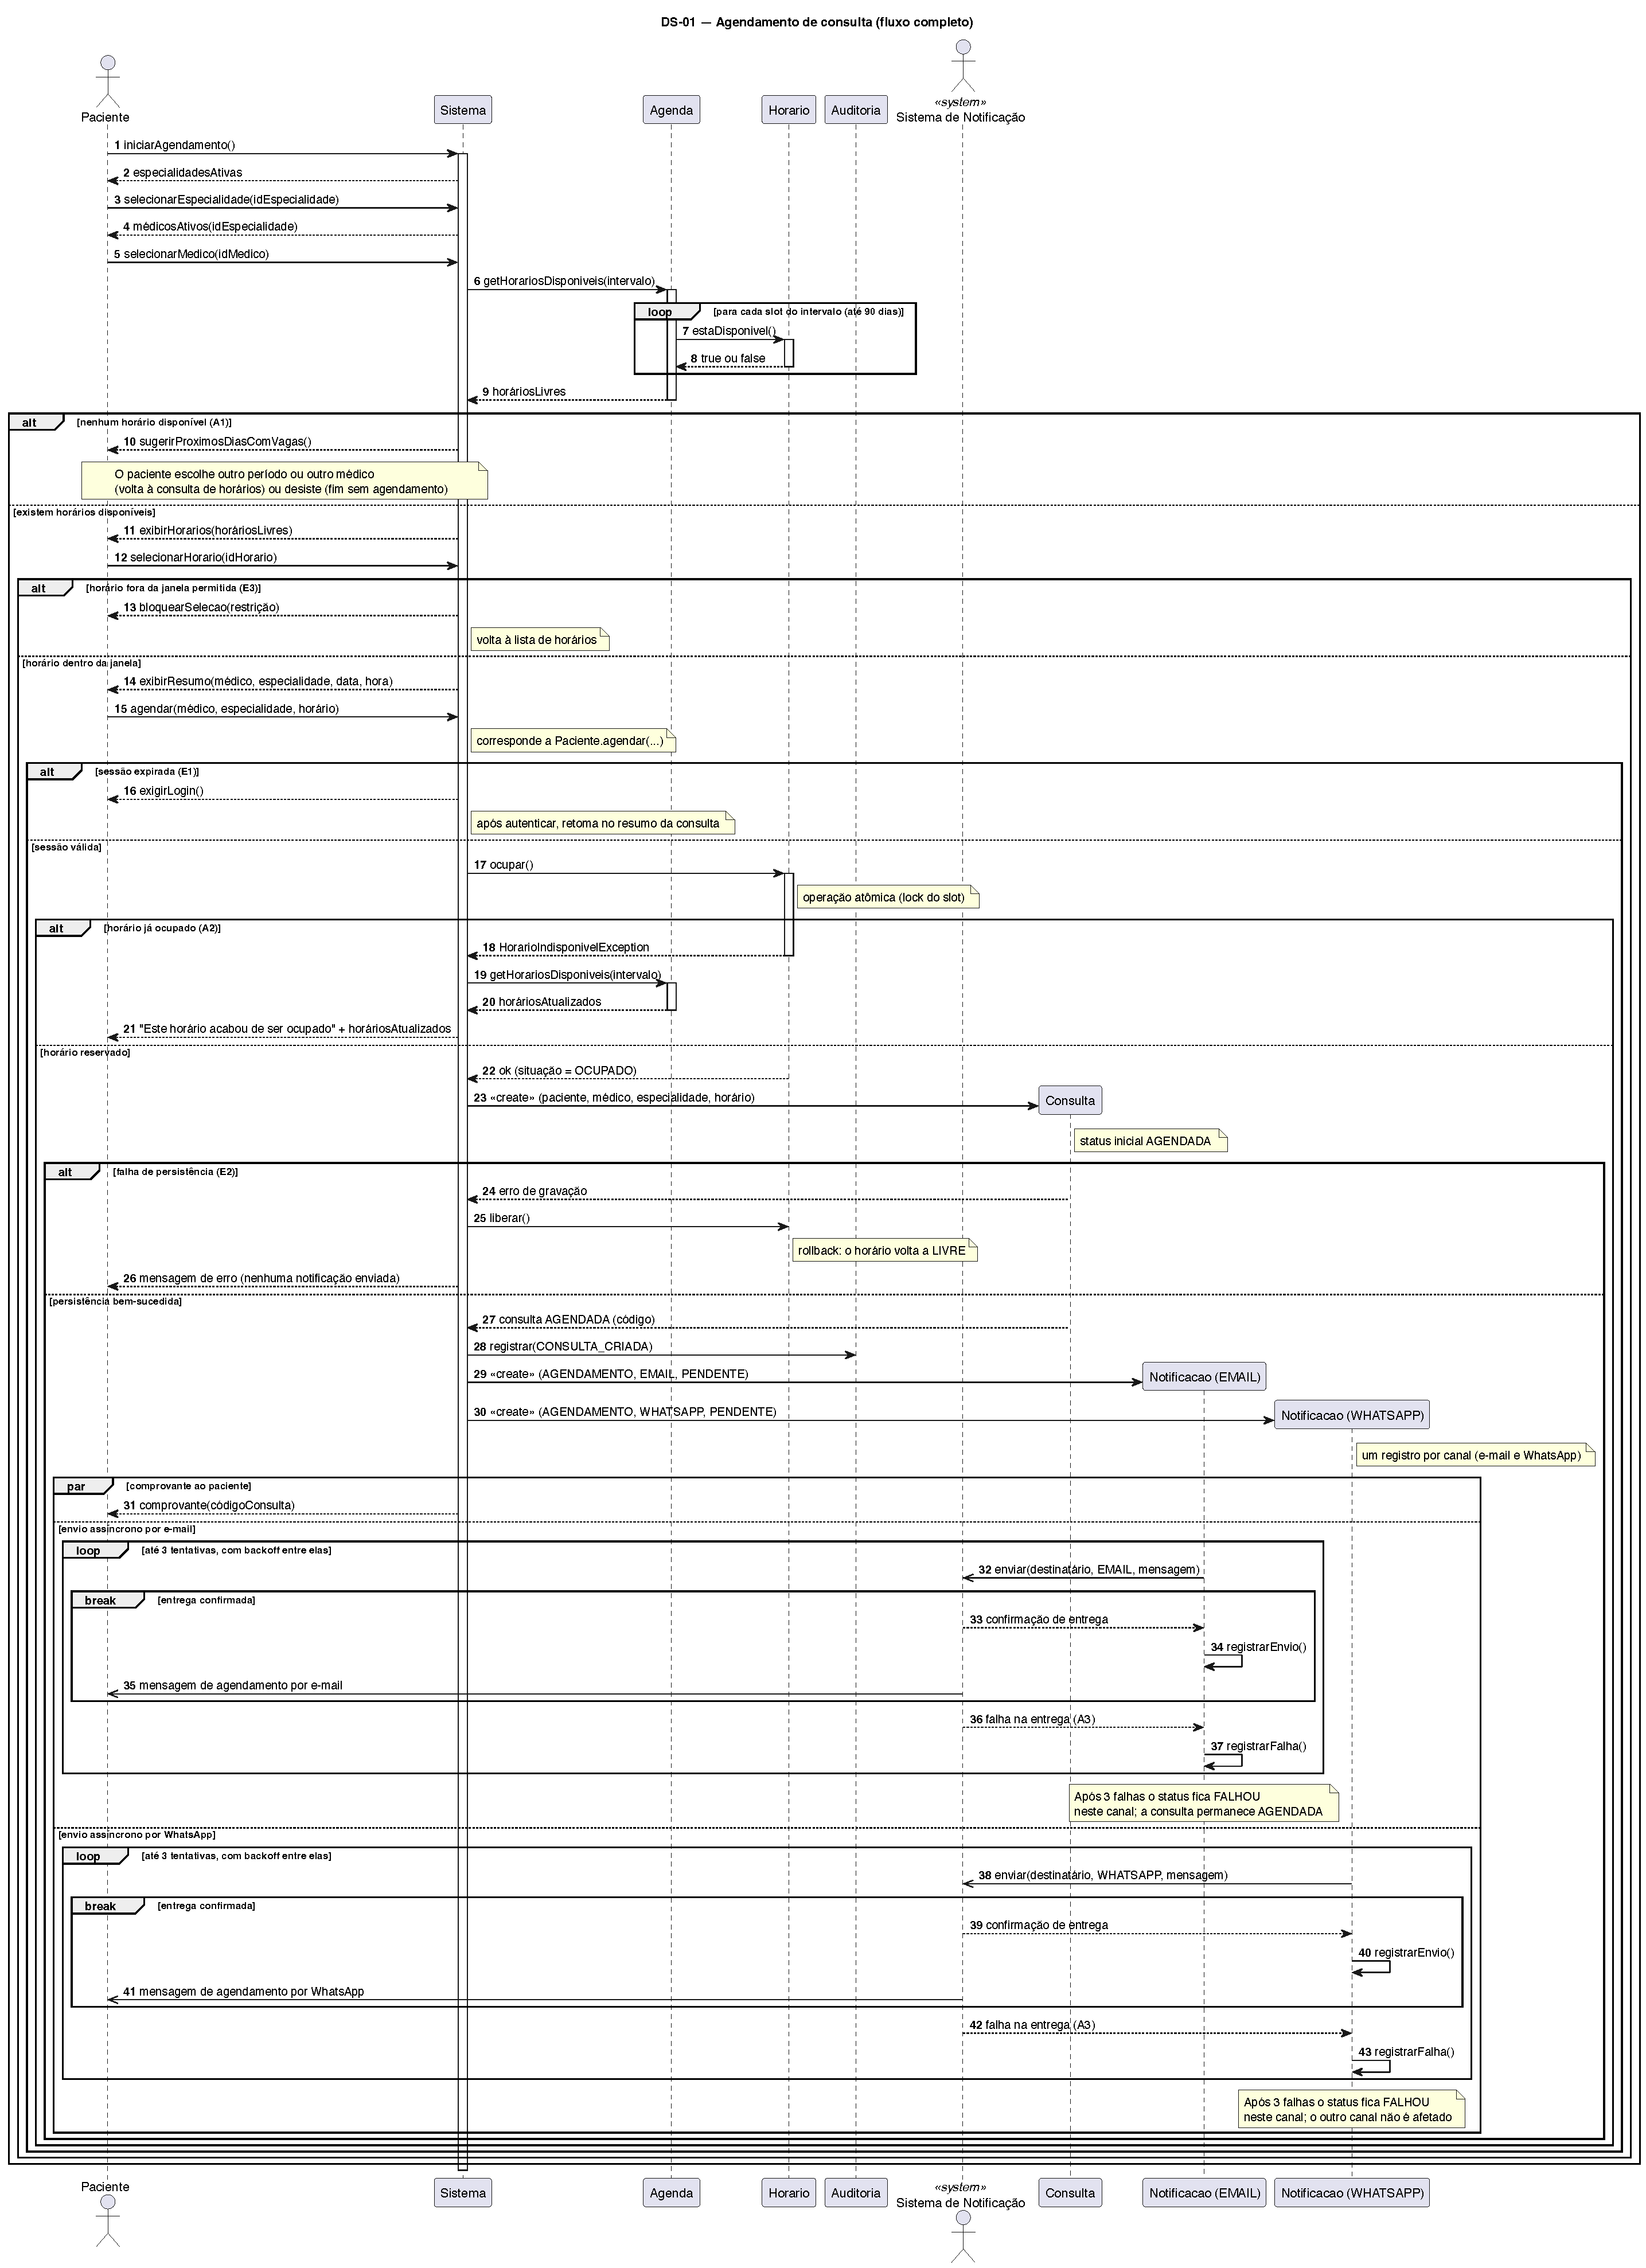
\includegraphics[width=\textwidth,height=5.8cm,keepaspectratio]{DS01_Agendamento.pdf}
\end{frame}

% Slide 12: DS-01 Reserva Atômica e Notificação
\setLayout{horizontal}
\begin{frame}{DS-01 --- Interação e Reserva Atômica}
    \begin{columns}
        \column{0.5\textwidth}
        \textbf{Objetos e Responsabilidades:}
        \begin{itemize}
            \item \textbf{Controlador Sistema:} orquestra tela e regras de negócio
            \item \textbf{Agenda / Horario:} verificação de grade e estado
            \item \textbf{Consulta / Notificacao:} instanciados dinamicamente (\texttt{<<create>>})
        \end{itemize}
        \vspace{0.4em}
        \textbf{Reserva Atômica (Mensagem 17):}
        \begin{itemize}
            \item \texttt{Horario.reservar()}: operação única atômica
            \item Elimina risco de \emph{race condition} no banco
        \end{itemize}

        \column{0.5\textwidth}
        \textbf{Rollback e Resiliência:}
        \begin{itemize}
            \item Mensagem 25: \texttt{Horario.liberar()} reverte o slot caso ocorra falha de gravação (E2)
        \end{itemize}
        \vspace{0.4em}
        \textbf{Paralelismo Concorrente:}
        \begin{itemize}
            \item Fragmento \texttt{par}: canais operam de modo independente
            \item Loop com até 3 tentativas e backoff em cada canal
            \item Comprovante na tela (msg 28) sem bloquear o paciente
        \end{itemize}
    \end{columns}
\end{frame}

% Slide 13: DS-01 Mapeamento Mensagens
\setLayout{vertical}
\begin{frame}{DS-01 --- Rastreabilidade de Mensagens e Cenários}
    \centering
    \resizebox{\textwidth}{!}{%
    \begin{tabular}{cll}
        \toprule
        \textbf{Mensagens} & \textbf{Cenário / Regra Coberta} & \textbf{Comportamento dos Objetos} \\
        \midrule
        1 a 8 & Autenticação e Catálogo & Paciente recebe lista de especialidades e médicos ativos \\
        9 a 12 & Consulta de Grade & \texttt{Agenda.getHorariosLivres()} --- trata \textbf{A1} (sem horários) \\
        13 a 16 & Validação da Janela e Sessão & Bloqueio se fora da janela (\textbf{E3}) e revalidação de sessão (\textbf{E1}) \\
        17 a 22 & Reserva e Conflito & \texttt{Horario.reservar()} --- trata \textbf{A2} (slot ocupado simultaneamente) \\
        23 a 28 & Persistência e Confirmação & Criação da \texttt{Consulta}, log em \texttt{Auditoria} e rollback (\textbf{E2}) \\
        29 a 45 & Notificação Concorrente & Bloco \texttt{par} (E-mail e WhatsApp) com loops de repetição (\textbf{A3}) \\
        \bottomrule
    \end{tabular}%
    }
\end{frame}

% ==========================================================
\section[DarkOrange]{Diagrama de Classes (DC)}

% Slide 14: DC Imagem
\setLayout{vertical}
\begin{frame}{DC --- Diagrama de Classes (Nível Macro)}
    \centering
    \vspace{0.1cm}
    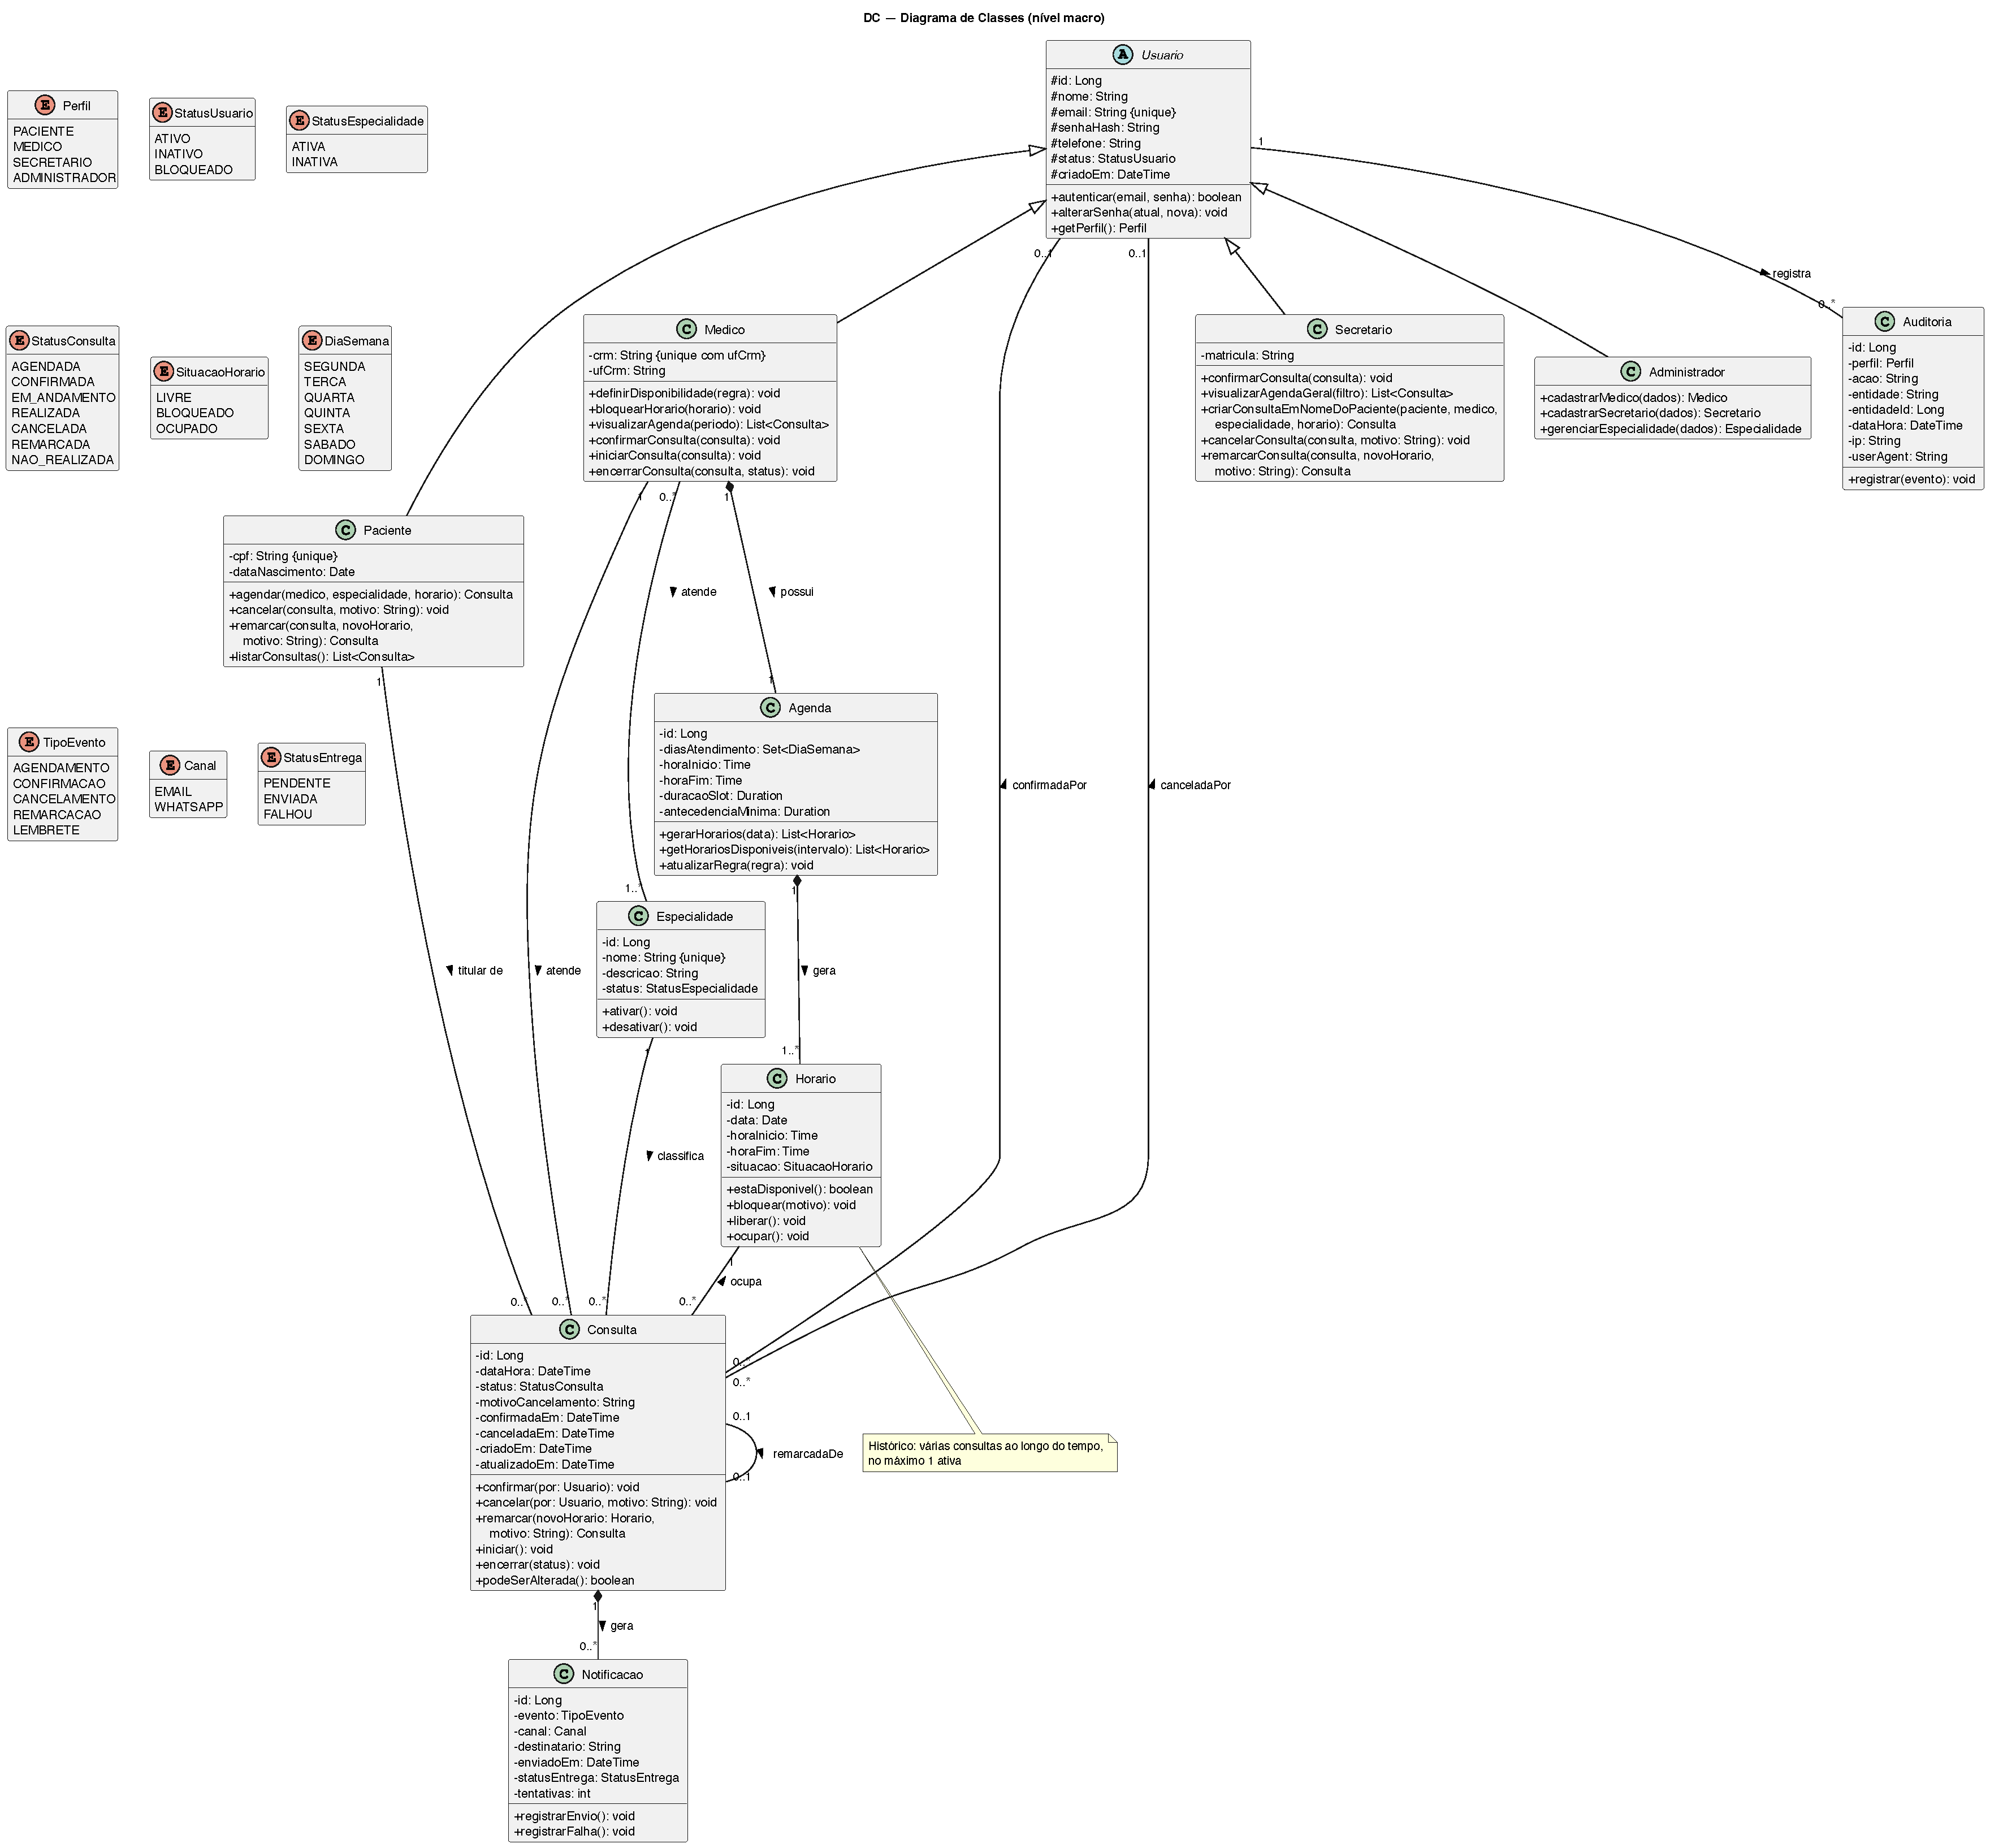
\includegraphics[width=\textwidth,height=5.8cm,keepaspectratio]{DC_Classes.pdf}
\end{frame}

% Slide 15: DC Herança e Perfis
\setLayout{horizontal}
\begin{frame}{DC --- Estrutura de Perfis e Herança}
    \begin{columns}
        \column{0.5\textwidth}
        \begin{block}{Classe Abstrata \texttt{Usuario}}
            Centraliza os atributos universais protegidos (\texttt{\#}):
            \begin{itemize}
                \item Identificação: \texttt{id}, \texttt{nome}, \texttt{telefone}
                \item Segurança: \texttt{email} \{unique\}, \texttt{senhaHash}
                \item Controle: \texttt{status}, \texttt{criadoEm}
                \item Métodos: \texttt{autenticar()}, \texttt{alterarSenha()}
            \end{itemize}
        \end{block}

        \column{0.5\textwidth}
        \textbf{Especialização dos Perfis:}
        \begin{itemize}
            \item \textbf{Paciente:} adiciona \texttt{cpf} \{unique\} e métodos de agendamento e cancelamento
            \item \textbf{Medico:} adiciona \texttt{crm}, \texttt{ufCrm} e controle de consultas
            \item \textbf{Secretario:} adiciona matrícula funcional e gestão de confirmações
            \item \textbf{Administrador:} métodos exclusivos para parametrização clínica
        \end{itemize}
    \end{columns}
\end{frame}

% Slide 16: DC Composições e Relacionamentos
\setLayout{horizontal}
\begin{frame}{DC --- Composições e Associações Críticas}
    \begin{columns}
        \column{0.5\textwidth}
        \textbf{Composições Estritas ($\blacklozenge$):}
        \begin{itemize}
            \item \textbf{Medico $\blacklozenge$ Agenda (1:1):} ciclo de vida dependente do vínculo médico
            \item \textbf{Agenda $\blacklozenge$ Horario (1:1..*):} slots pertencem unicamente à agenda-mãe
            \item \textbf{Consulta $\blacklozenge$ Notificacao (1:0..*):} registros de envio vinculados à consulta
        \end{itemize}

        \column{0.5\textwidth}
        \textbf{Associações Estruturais:}
        \begin{itemize}
            \item \textbf{Horario -- Consulta (1:0..*):} slot retém histórico completo (máx. 1 consulta ativa)
            \item \textbf{Consulta -- Consulta (0..1:0..1):} autoassociação reflexiva \texttt{remarcadaDe}
            \item \textbf{Usuario -- Auditoria (1:0..*):} associação simples para perenidade dos logs (LGPD)
        \end{itemize}
    \end{columns}
\end{frame}

% Slide 17: DC Enumerações
\setLayout{horizontal}
\begin{frame}{DC --- Domínios Blindados (9 Enumerações)}
    \begin{columns}
        \column{0.5\textwidth}
        \textbf{Controle de Acesso e Entidades:}
        \begin{itemize}
            \item \texttt{Perfil}: restringe contas a 4 perfis estritos
            \item \texttt{StatusUsuario}: \texttt{ATIVO}, \texttt{INATIVO}, \texttt{BLOQUEADO}
            \item \texttt{StatusEspecialidade}: \texttt{ATIVA}, \texttt{INATIVA}
            \item \texttt{DiaSemana}: parametrização da grade do médico
        \end{itemize}

        \column{0.5\textwidth}
        \textbf{Estados Clínicos e Mensageria:}
        \begin{itemize}
            \item \texttt{StatusConsulta}: 7 estados do ciclo de vida
            \item \texttt{SituacaoHorario}: \texttt{LIVRE}, \texttt{BLOQUEADO}, \texttt{OCUPADO}
            \item \texttt{TipoEvento}: gatilhos padronizados de disparo
            \item \texttt{Canal}: \texttt{EMAIL} ou \texttt{WHATSAPP}
            \item \texttt{StatusEntrega}: \texttt{PENDENTE}, \texttt{ENVIADA}, \texttt{FALHOU}
        \end{itemize}
    \end{columns}
\end{frame}

% ==========================================================
\section[DarkGreen]{Considerações Finais}

% Slide 18: Síntese e Resultados
\setLayout{horizontal}
\begin{frame}{Síntese e Decisões de Modelagem}
    \begin{columns}
        \column{0.5\textwidth}
        \textbf{Consistência e Qualidade:}
        \begin{itemize}
            \item 100\% de rastreabilidade entre RFs, RNs e diagramas UML
            \item Eliminação de concorrência com reserva atômica de slots
            \item Modelo desacoplado para notificações assíncronas
            \item Domínio fortemente tipado sem strings mágicas
        \end{itemize}

        \column{0.5\textwidth}
        \textbf{Conformidade e Extensibilidade:}
        \begin{itemize}
            \item Diagramação aderente ao padrão UML 2.5
            \item Rastreabilidade de auditoria em conformidade com LGPD
            \item Base sólida para evolução arquitetural (ex: pagamentos, telemedicina e filas de espera)
        \end{itemize}
    \end{columns}
\end{frame}

% Slide 19: Conclusão / Dúvidas
\setLayout{blank}
\setBGColor{UFGBlue}
\begin{frame}[noframenumbering]{}
    \centering
    \vspace{1.5cm}
    {\Huge \textbf{Obrigado!}}\\[1.0cm]
    {\Large Sistema de Agendamento de Consultas Médicas}\\[0.4cm]
    {\normalsize Modelagem de Software --- APS 1 | UFG / INF (2026/2)}\\[1.2cm]
    {\large \textbf{Dúvidas e Discussão}}
\end{frame}

\end{document}
